\documentclass[11pt,fleqn,report,uplatex]{jsbook}

\usepackage[dvipdfm]{graphicx} % 画像の挿入
\usepackage{amsmath} % 数式のサポート
\usepackage{bm} % 太字の数式
\usepackage{here} % 図や表の位置指定
\usepackage{float} % 図や表の位置指定
\usepackage{booktabs} % 表の装飾
\usepackage{array} % 配列の高さ設定
\usepackage{multirow} % 表の行結合
\usepackage{txfonts} % Timesフォントの使用
\usepackage{pifont} % 丸付き文字
\usepackage{cite} % 参考文献の引用
\usepackage{siunitx} % 単位の記載
\usepackage[hang,small,bf]{caption} % キャプションの設定
\usepackage[subrefformat=parens]{subcaption} % サブキャプションの設定
\captionsetup{compatibility=false}
\usepackage[dvipdfmx]{hyperref} % ハイパーリンクの設定
\usepackage{fancyhdr} % ヘッダーの設定

\numberwithin{equation}{chapter} % 数式番号を章ごとにリセット
\numberwithin{figure}{chapter} % 図番号を章ごとにリセット
\numberwithin{table}{chapter} % 表番号を章ごとにリセット
\renewcommand{\figurename}{Fig.\ } % 図のキャプションをFig.に変更
\renewcommand{\tablename}{Table\ } % 表のキャプションをTableに変更
\setlength{\baselineskip}{10pt} % 行間の設定

\setcounter{tocdepth}{2} % 目次の深さ設定

\def\theequation{\thechapter.\arabic{equation}} % 数式番号のスタイル設定

\makeatletter
    \DeclareRobustCommand\cite{\unskip
\@ifnextchar[{\@tempswatrue\@citex}{\@tempswafalse\@citex[]}}
    \def\@cite#1#2{$^{\hbox{\scriptsize({#1\if@tempswa , #2\fi})}}$}
    \def\@biblabel#1{(#1)}
\makeatother

\setlength{\mathindent}{2zw} % 数式のインデント設定

\renewcommand{\thefigure}{\thechapter.\arabic{figure}} % 図番号のスタイル設定
\renewcommand{\thetable}{\thechapter.\arabic{table}} % 表番号のスタイル設定

\hypersetup{
    setpagesize=false,
    bookmarksnumbered=true,
    bookmarksopen=true,
    colorlinks=true,
    linkcolor=black,
    citecolor=black,
}
\pagestyle{fancy}
    \chead{} % 中央ヘッダーの設定
    \lhead[]{\leftmark} % 左ヘッダーの設定
    \rhead[\rightmark]{} % 右ヘッダーの設定

\renewcommand{\chaptermark}[1]{\markboth{第\ \thechapter\ 章  ~#1}{}}
\renewcommand{\sectionmark}[1]{\markright{\thesection  #1}{}}

% 設定ここまで

\begin{document}

\frontmatter % タイトルと目次
\pagestyle{empty}

\include{chapters/title}

\tableofcontents

\mainmatter % 本文
\pagestyle{fancy}

\section[Test]{Test}
test\cite{example}

\begin{equation}
    \label{eq:test}
    a = b
\end{equation}

\begin{figure}[H]
    \centering
    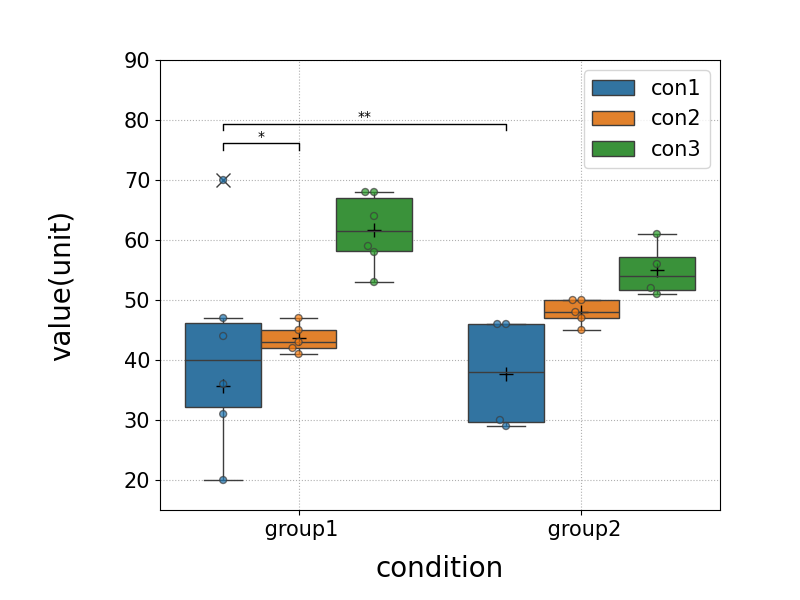
\includegraphics[width=\textwidth]{figures/test/test.png} % サイズを指定
    \caption{Test}
    \label{fig:test}
\end{figure}

\begin{table}[H]
    \centering
    \caption{Test}
    \label{tab:test}
    \begin{tabular}{|c|c|}
        \hline
        a & b \\
        \hline
    \end{tabular}
\end{table}
 % テスト用の章

\section{Introduction}

aaa\cite{example}


\bibliographystyle{junsrt} % 参考文献スタイル
\bibliography{bibliography/reference} % 参考文献リストの表示

\end{document}
